\section{Problems with hyperbolic space} \label{sec:hyperbolic_problems}
As described in \autoref{subsec:practical_considerations}, in hyperbolic geometry the world moves and the camera is stationary.
This is done to limit the distortions, since the distortions get bigger the further away from $(0,0,0)$ the object is.
In first-person the camera is normally where head of the player is.
However, if we were to place the camera there in hyperbolic geometry, the distortions would be very small, barely distinguishable from Euclidean geometry as can be seen in \autoref{fig:hyperbolic_invisible}.

\begin{figure}[h]
    \centering
    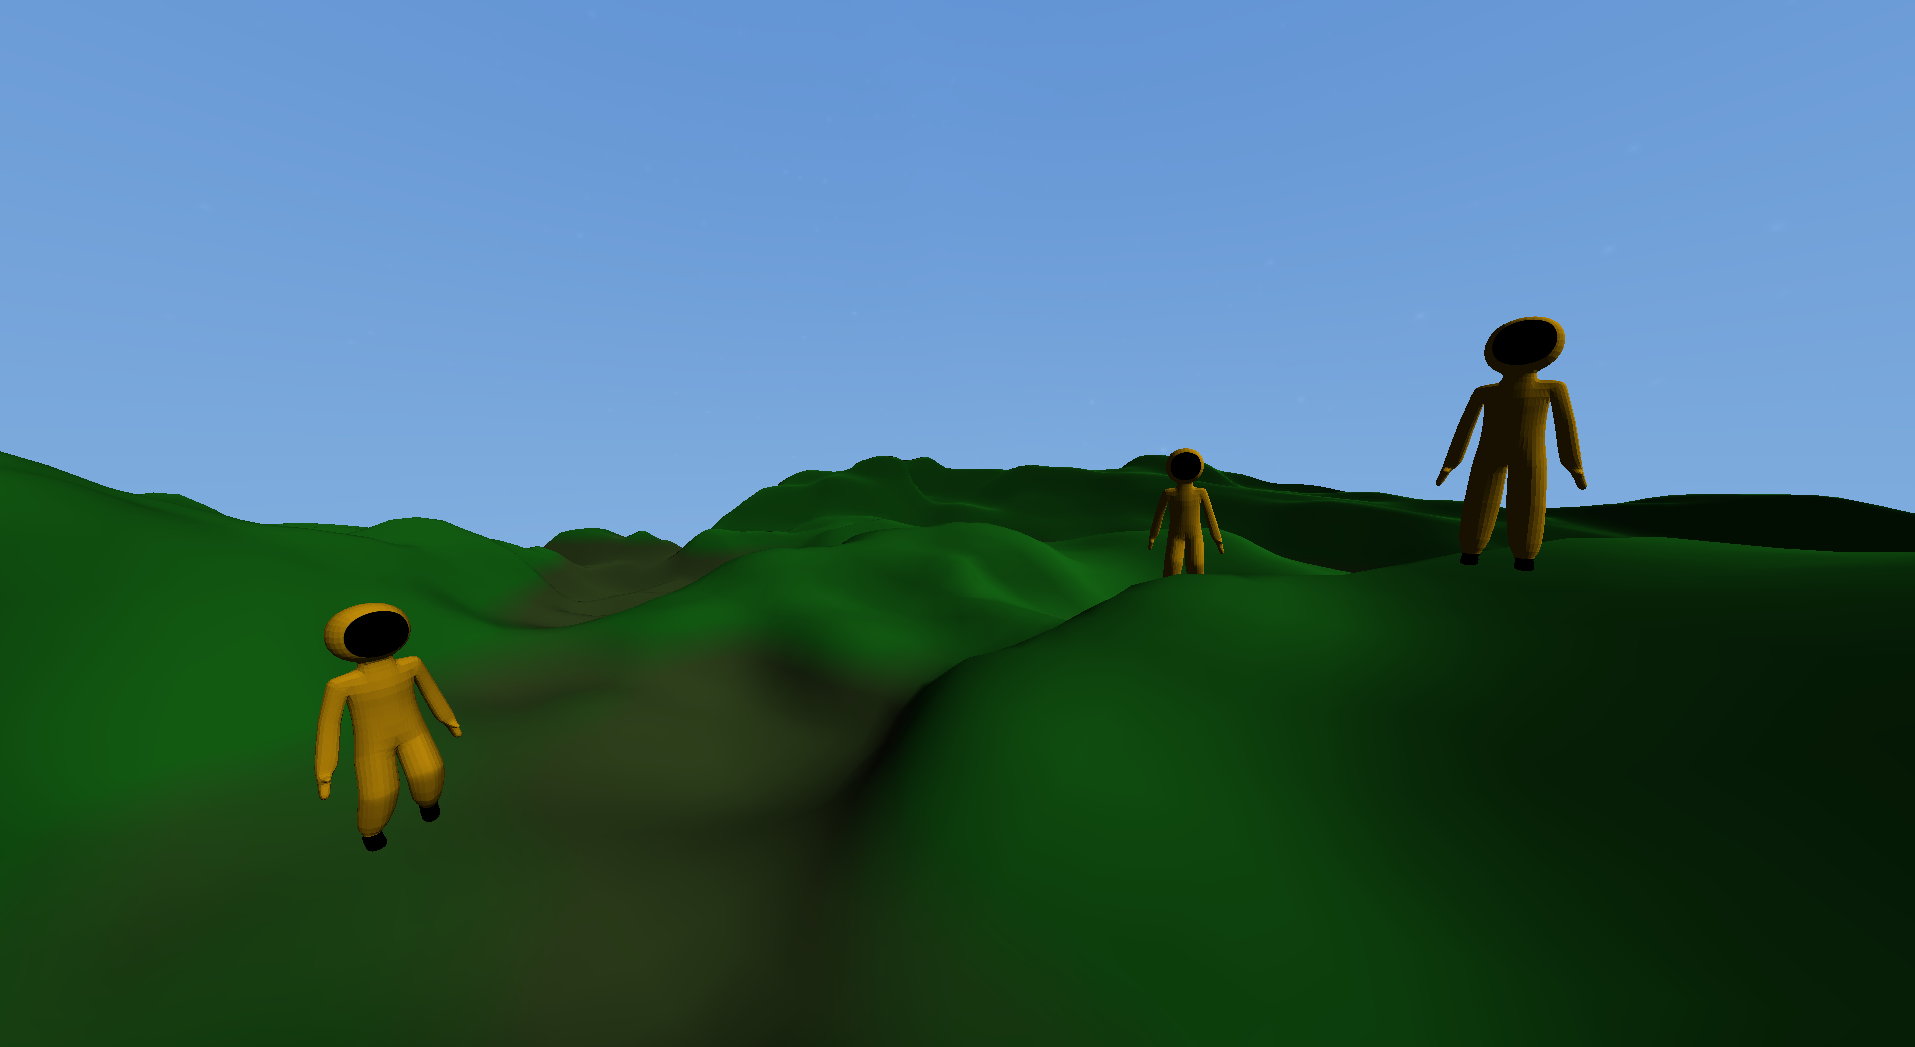
\includegraphics[width=0.8\textwidth]{chapters/problems/resources/hyperbolic-invisible.png}
    \caption{Hyperbolic geometry with camera at player's head.}
    \label{fig:hyperbolic_invisible}
\end{figure}

To make the distortions more visible, the camera was placed high above the player.
This solution, however, created a new problem.
The camera was too high which made gameplay look unnatural, which can be seen in \autoref{fig:hyperbolic_high_camera}.

\begin{figure}[h]
    \centering
    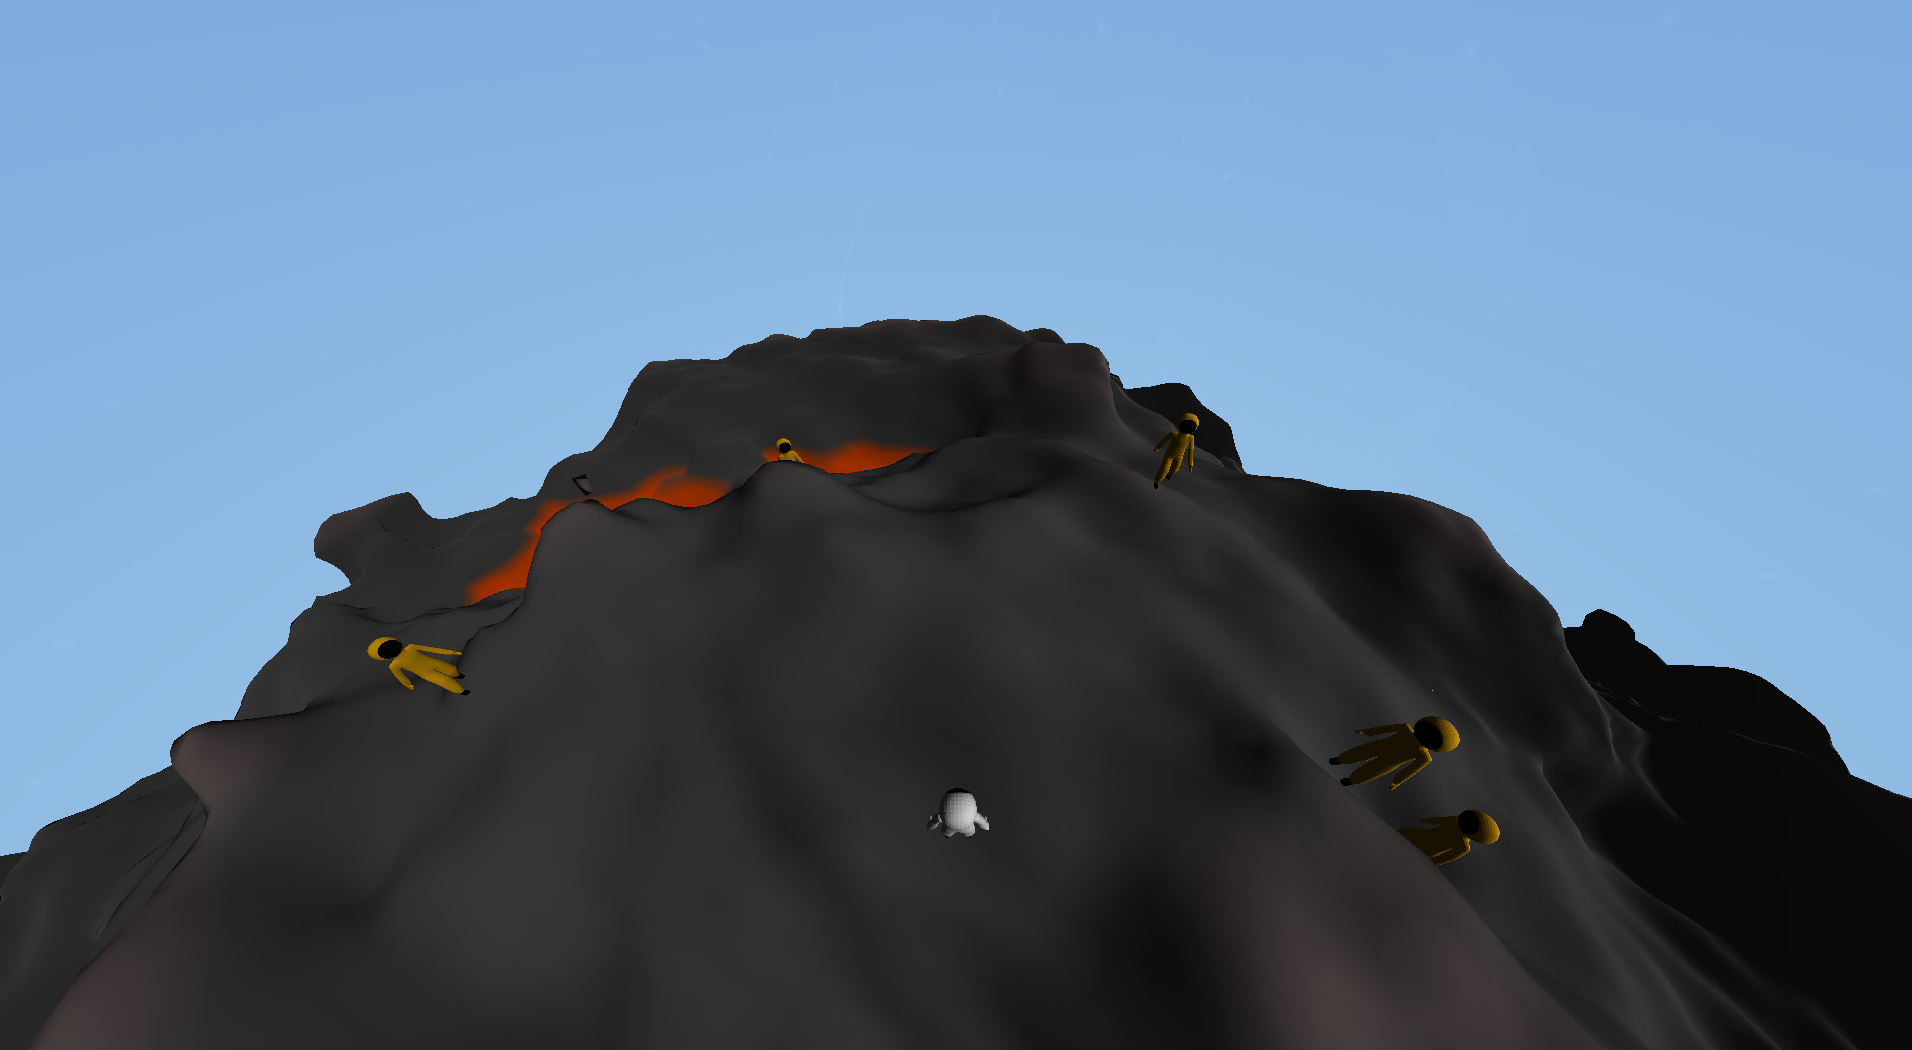
\includegraphics[width=0.8\textwidth]{chapters/problems/resources/hyperbolic-high-camera.png}
    \caption{Hyperbolic camera placed high above the player.}
    \label{fig:hyperbolic_high_camera}
\end{figure}

The solution to this problem was to move the whole world up.
The whole logic is as follows:
\begin{enumerate}
    \item The player inputs a key combination that moves him.
    \item The world is moved to simulate the effect of the player moving.
    \item The world is moved up to adjust for the raised camera.
    \item The frame is rendered.
\end{enumerate}

It is worth noting that moving the world only involves passing an appropriate vector to the shader.
The locations of the objects themselves are not changed for performance reasons.